\section{Don't Augment Me - appendix}\label{appendix:dont-augment}

\subsection{SSIM attribution ranges}\label{appendix:ssim-ranges}

\begin{table}[h]
 \centering
  \caption{SSIM ranges for attribution methods for ResNet18}
  \label{tab:ranges-for-resnet}
    \begin{tabular}{|l|lllll|}
    \hline
     \backslashbox{Attribution}{Dataset} & Edible plants & Food 101 & Marvel & Plants &
     Stanford Dogs \\
     \hline
    Deconvolution & 0.784622 & 0.423285 & 0.473029 & 0.682504 & 1.283490\\
    Integrated Gradients & 0.421971 & 1.306827 & 0.611498 & 0.887589 & 1.565911\\
    Saliency & 0.047666 & 0.045500 & 0.067406 & 0.094456 & 0.060711\\
    Grad-Cam  & 0.000047 & 0.000051 & 0.000022 & 0.000085 & 0.000064 \\
    Grad-Shap & 0.145404 & 0.093035 & 0.102947 & 0.285072 & 0.147860 \\
    Guided Backprop & 0.079774 & 0.069185 & 0.050991 & 0.126553 & 0.152545 \\
    \hline
    \end{tabular}
\end{table}


\begin{table}[h]
 \centering
  \caption{SSIM ranges for attribution methods for DenseNet121}
  \label{tab:ranges-for-densenet}
    \begin{tabular}{|l|lllll|}
    \hline
     \backslashbox{Attribution}{Dataset} & Edible plants & Food 101 & Marvel & Plants &
     Stanford Dogs \\
     \hline
    Deconvolution & 4677.117 & 80.11916 & 3037.732 & 1715.939 & 2044.188\\
    Integrated Gradients & 1.099644 & 2.577734 & 0.997656 & 0.816421 & 2.090753\\
    Saliency & 0.068720 & 0.048571 & 0.052243 & 0.068942 & 0.149736\\
    Grad-Cam  & 0.000278 & 0.000187 & 0.000510 & 0.000395 & 0.002106 \\
    Grad-Shap & 0.142074 & 0.119778 & 0.162216 & 0.143393 & 0.345822\\
    Guided Backprop & 0.400560 & 0.218944 & 0.512460 & 0.720738 & 1.565153\\
    \hline
    \end{tabular}
\end{table}

\begin{table}[h]
 \centering
  \caption{SSIM ranges for attribution methods for EfficientNet B0}
  \label{tab:ranges-for-efficientnet}
    \begin{tabular}{|l|lllll|}
    \hline
     \backslashbox{Attribution}{Dataset} & Edible plants & Food 101 & Marvel & Plants &
     Stanford Dogs \\
     \hline
    Deconvolution & 0.078107 & 0.025042 & 0.030603 & 0.055335 & 0.071512\\
    Integrated Gradients & 0.732469 & 5.059399 & 0.810054 & 1.551912 & 2.329165\\
    Saliency & 0.095080 & 0.032253 & 0.043658 & 0.140426 & 0.136111\\
    Grad-Cam  & 0.000028 & 0.000005 & 0.000007 & 0.000042 & 0.000037 \\
    Grad-Shap & 0.464270 & 0.054290 & 0.154112 & 0.280005 & 0.352823\\
    Guided Backprop & 0.068730 & 0.037462 & 0.030622 & 0.066075 & 0.102107\\
    \hline
    \end{tabular}
\end{table}

\subsection{Detailed SSIM results}

\begin{figure}[ht]
  \centering
  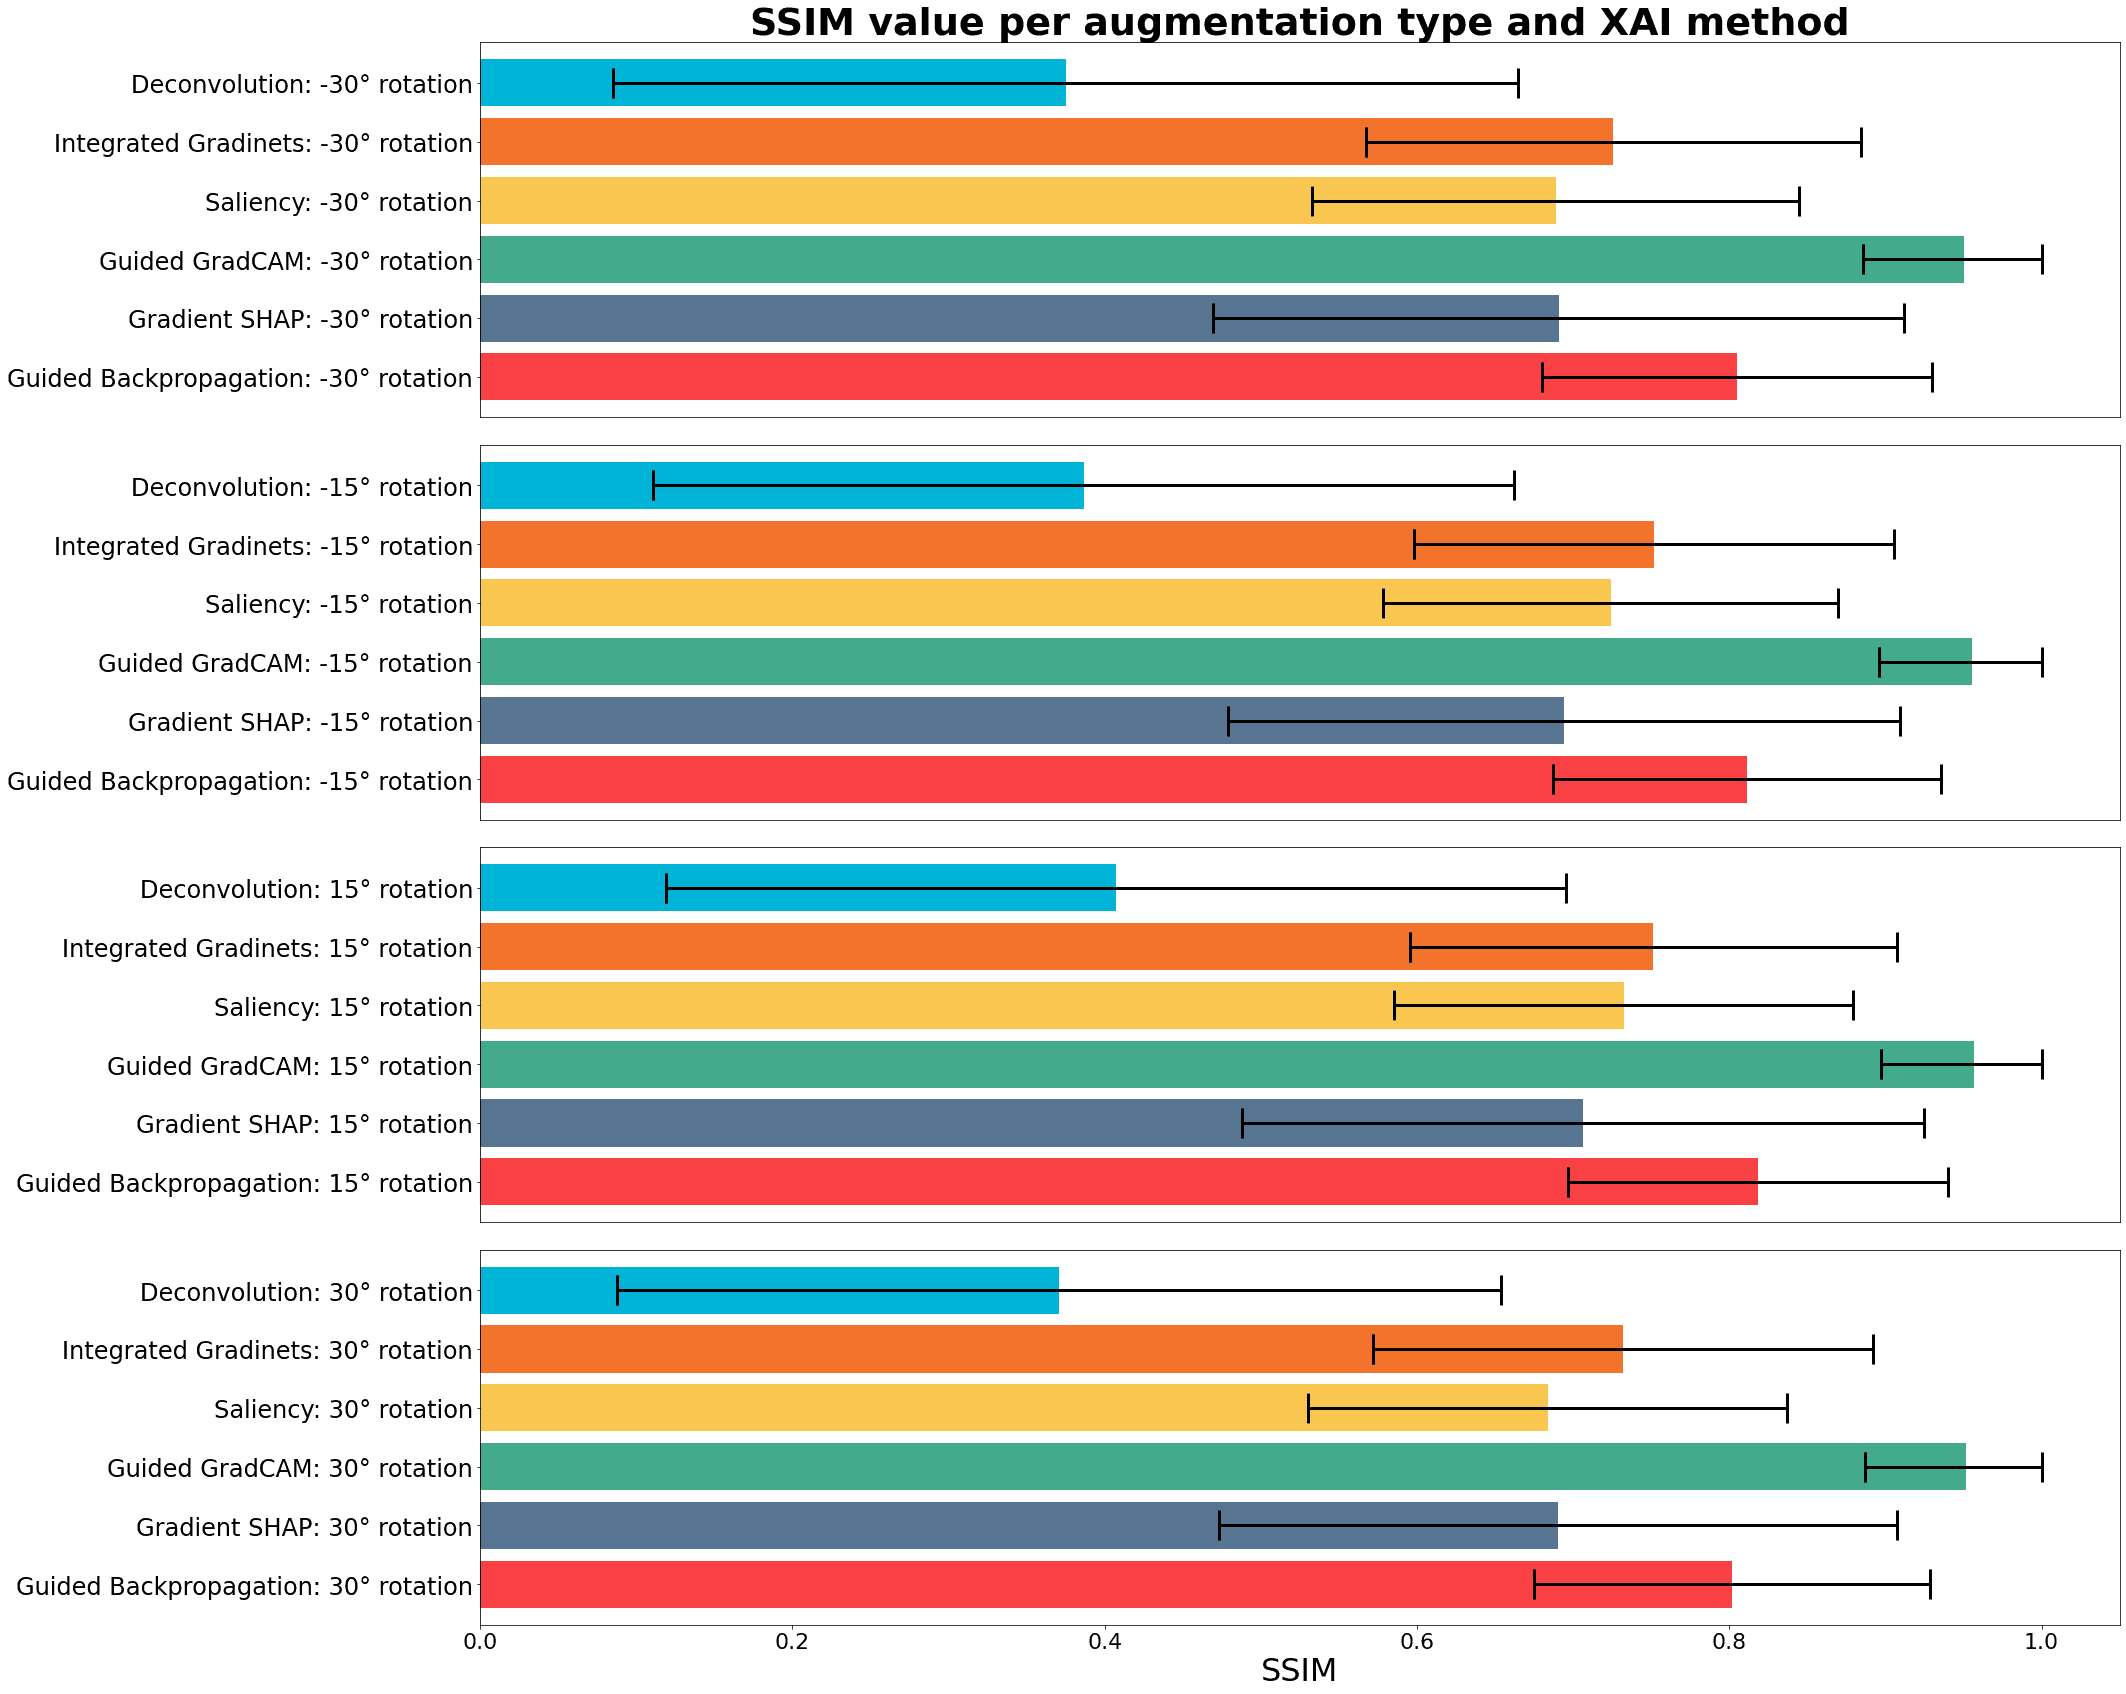
\includegraphics[width=\textwidth]{appendixes/images/rotation-ssim.png}
  \caption{Average SSIM values per attribution method and augmentation type (rotations). Each bar represents a methods' mean value of SSIM. Values used to calculate the mean value are restricted to come only from images augmented by applying specific rotations.}\label{fig:SSIM-all-rotation}
\end{figure}

\begin{figure}[ht]
  \centering
  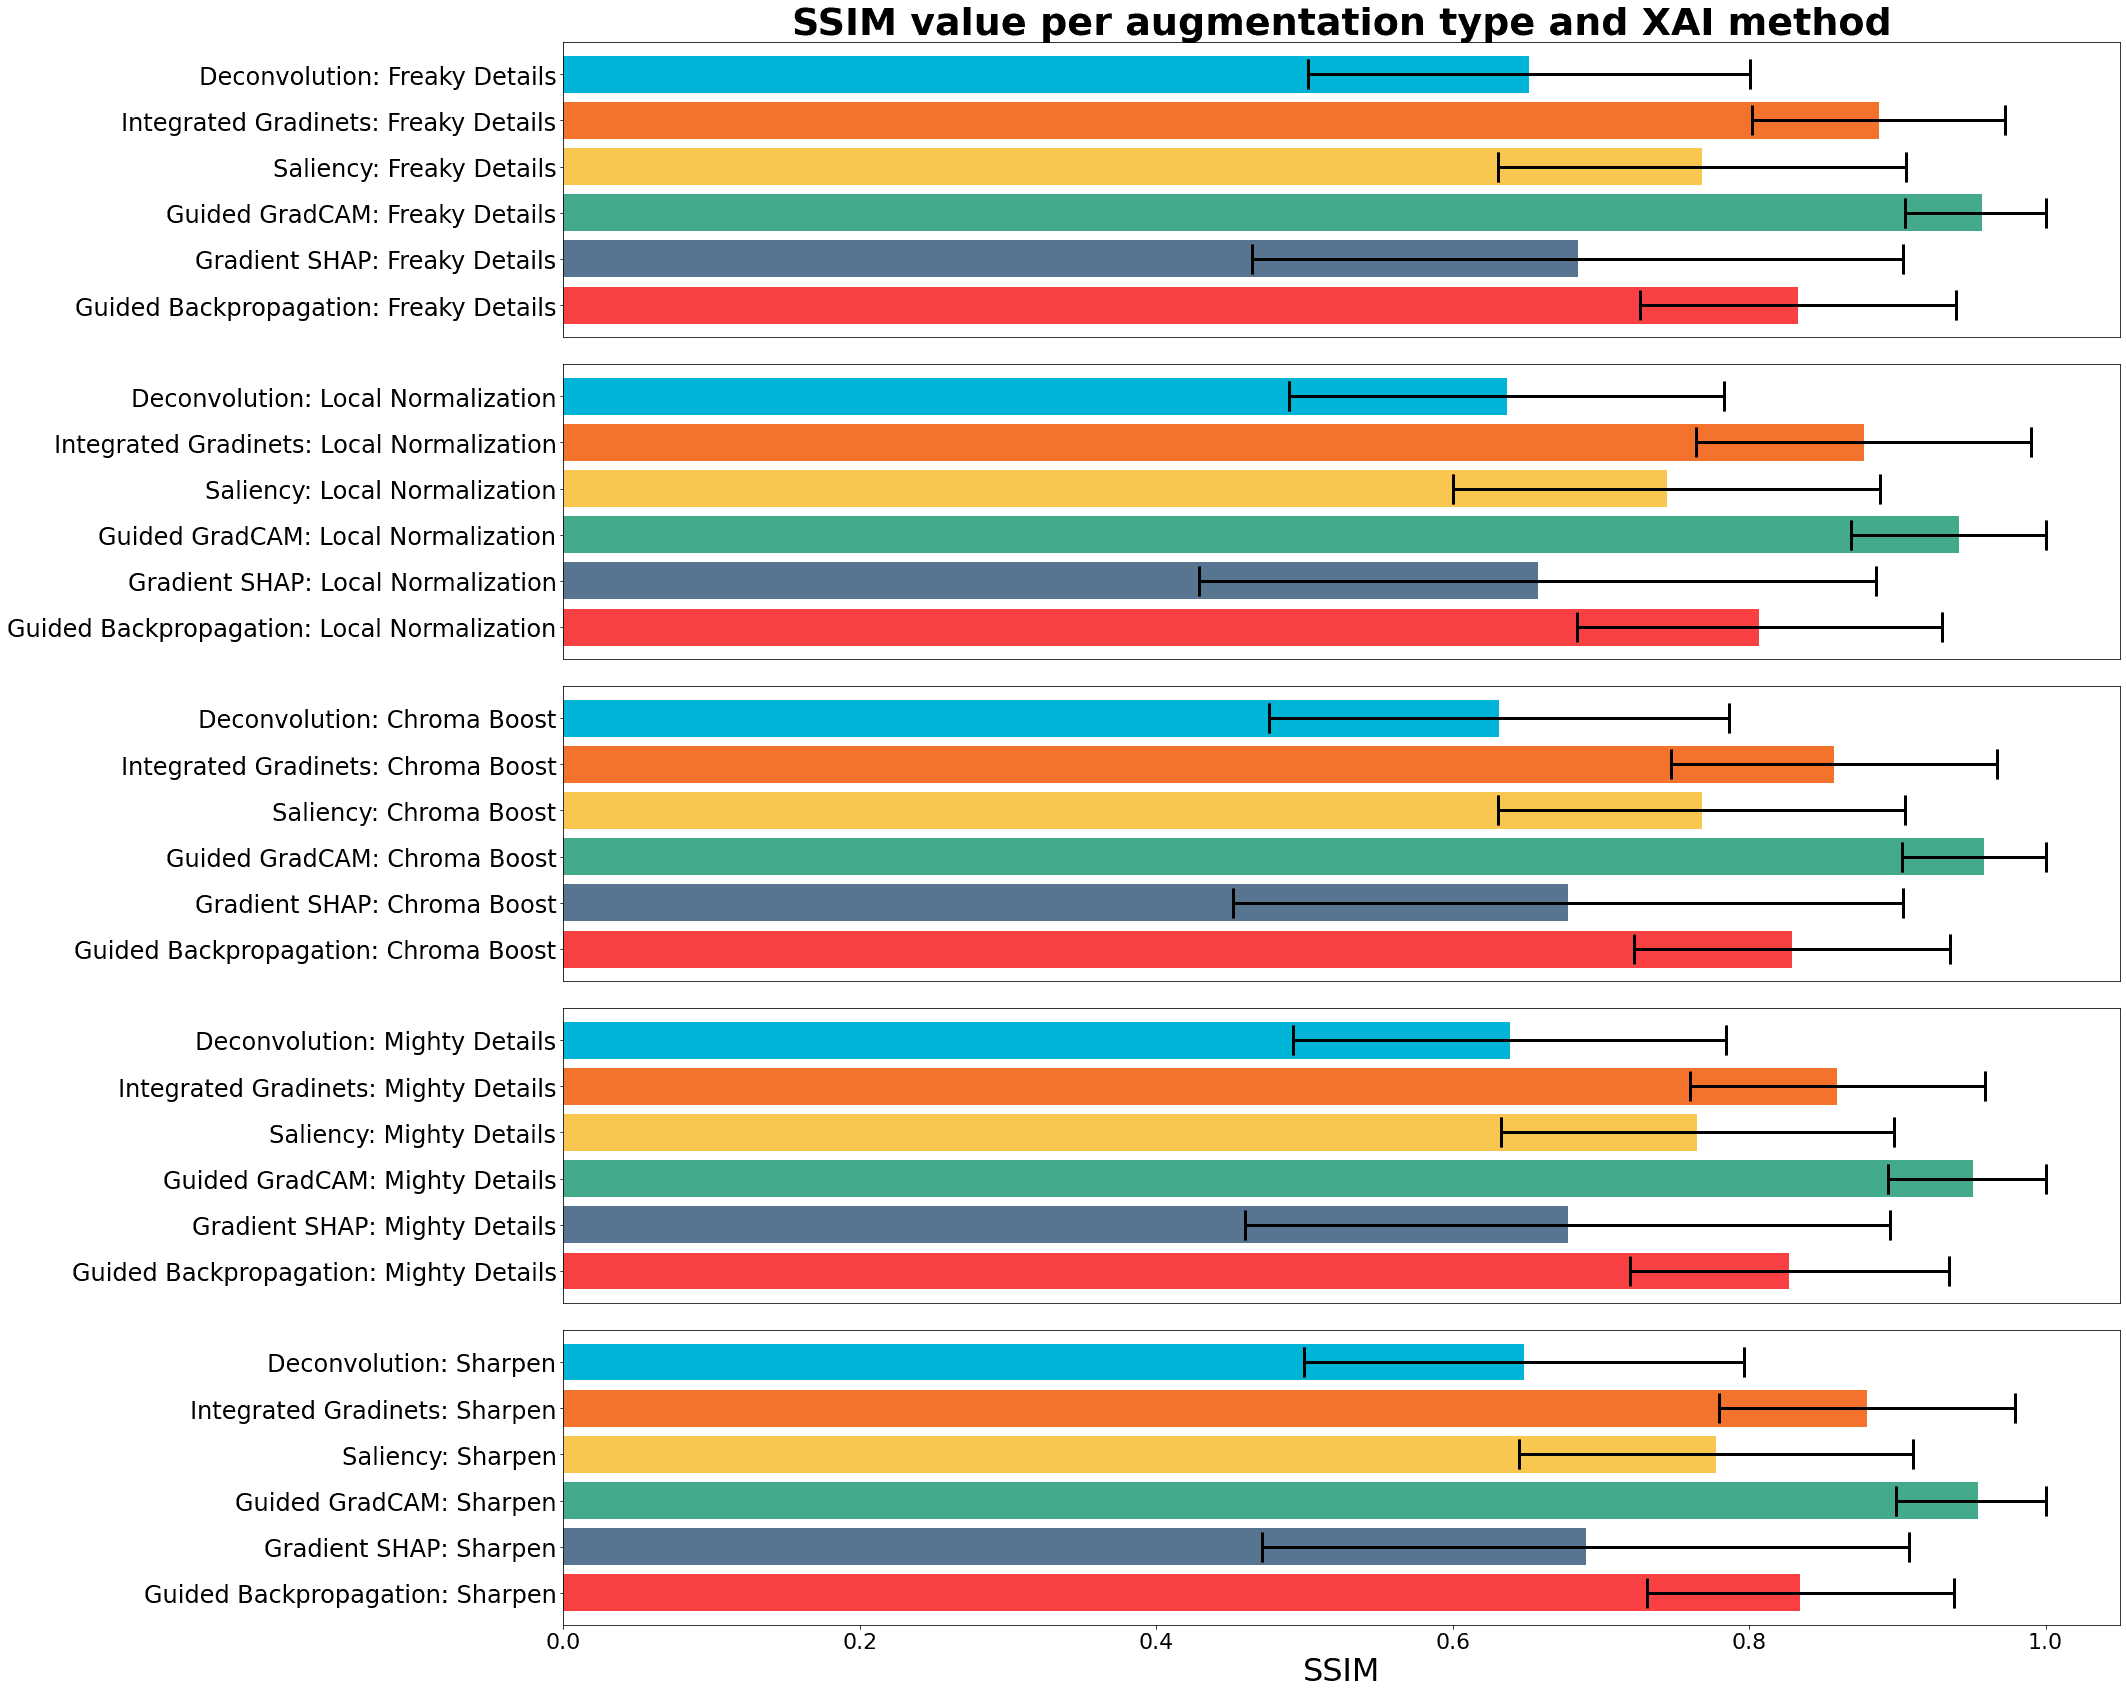
\includegraphics[width=\textwidth]{appendixes/images/filters-ssim.png}
  \caption{Average SSIM values per attribution method and augmentation type (filters). Each bar represents a methods' mean value of SSIM. Values used to calculate the mean value are restricted to come only from images augmented by applying specific filter.}\label{fig:SSIM-all-filters}
\end{figure}

\FloatBarrier

\subsection{Attributions samples}\label{appendix:attribution-samples}

Because the amount of attribution examples is to large to fit them in the appendix, they are available at \url{https://drive.google.com/drive/folders/1Vp3MYRg8j-6ZAfDePeT5kHYPu2Rv6r4t?usp=sharing} (total number of files equals $97990$). File structure is following the pattern \verb|{Augmentation Type}/{Dataset}/{Model version}/{XAI method}|. Each image has a filename containing:

\verb|{index}-{sample id}-{class id}-{augmentation method}-{true class}-{predicted class}.png|

\vspace{5mm}

Combined attribution samples are available at

\url{https://drive.google.com/drive/folders/1lnNQwH3-H1cHiNOEcmnd4OhSScDSuzt0?usp=sharing}.

\begin{figure}[ht]
  \centering
  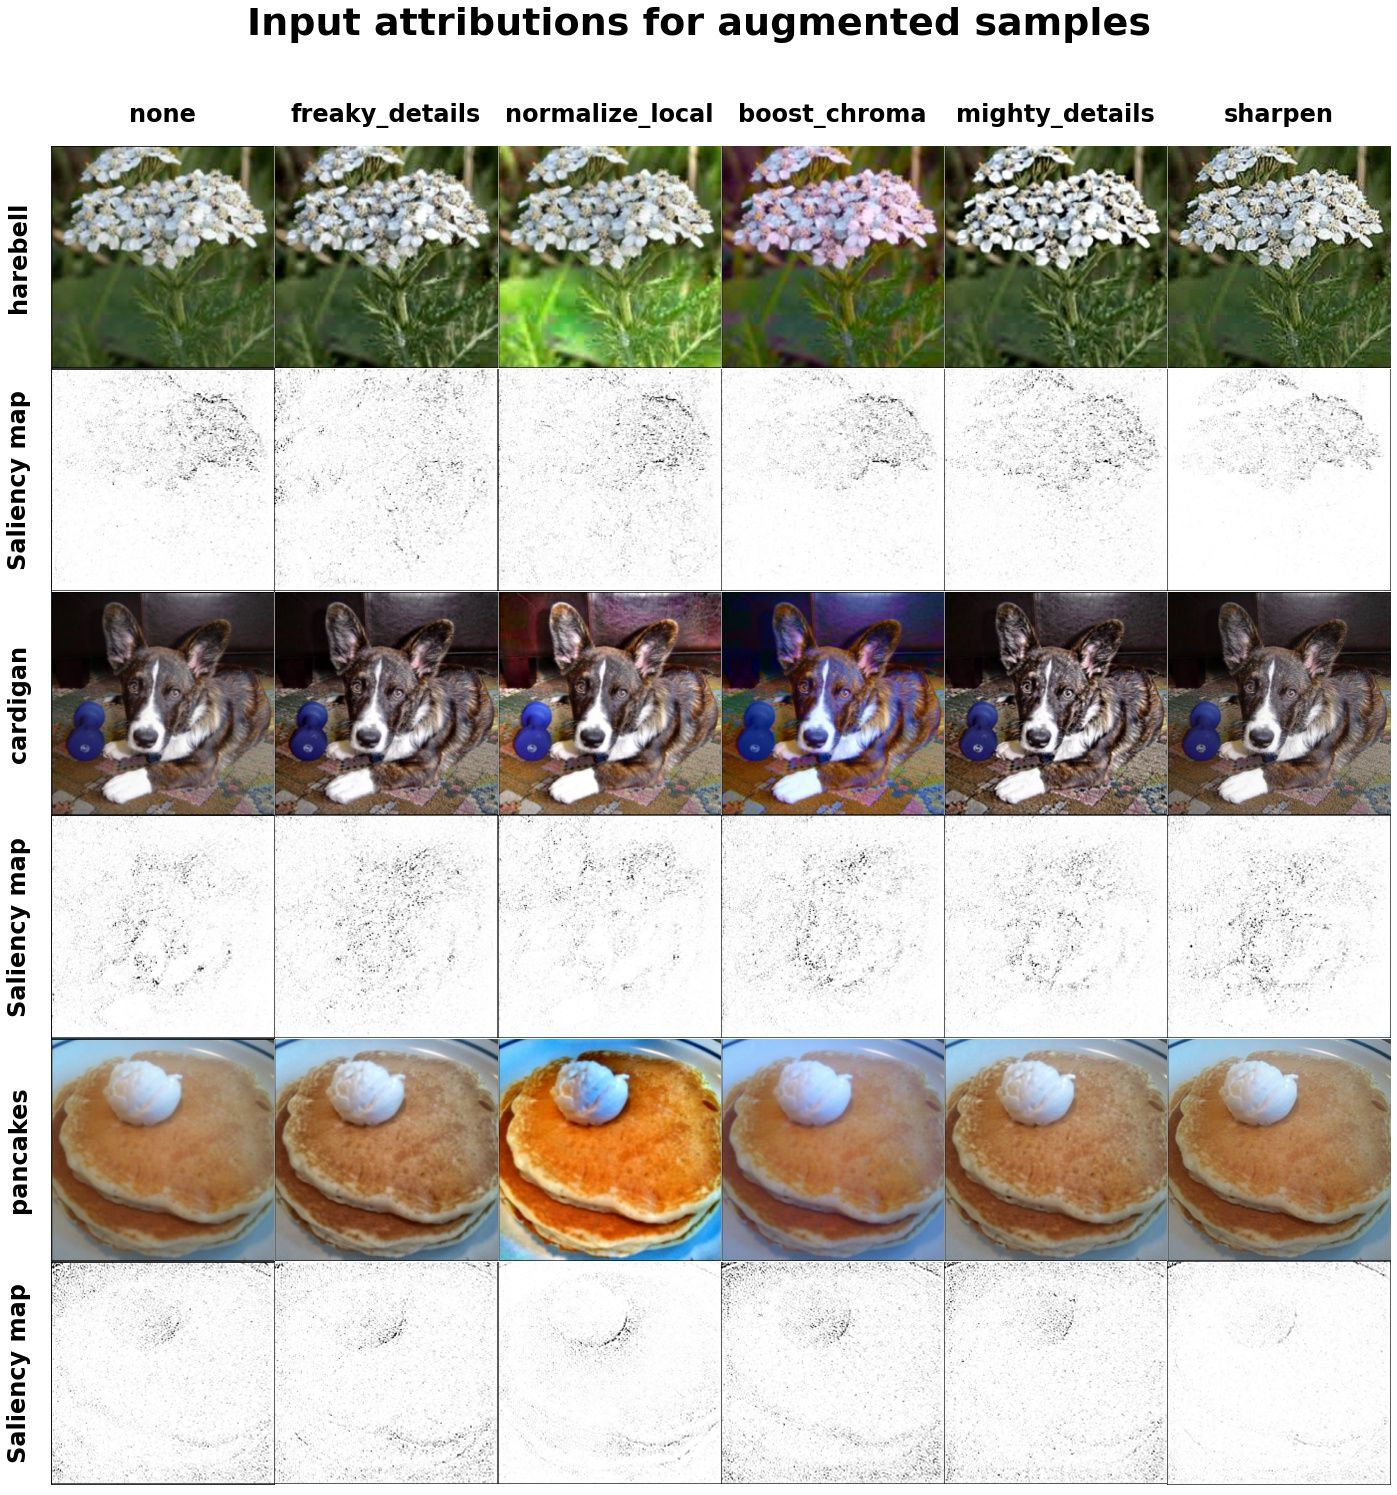
\includegraphics[width=0.8\textwidth]{appendixes/images/filters-sample.jpg}
  \caption{\textbf{Attribution comparison of inputs with applied filters.} Figure shows three distinct images (\textit{harebell\_flower}, \textit{cardigan}, \textit{pancakes}) with different filters. All attributions done by Guided GradCAM.}\label{fig:filters-samples}
\end{figure}

\begin{figure}[ht]
  \centering
  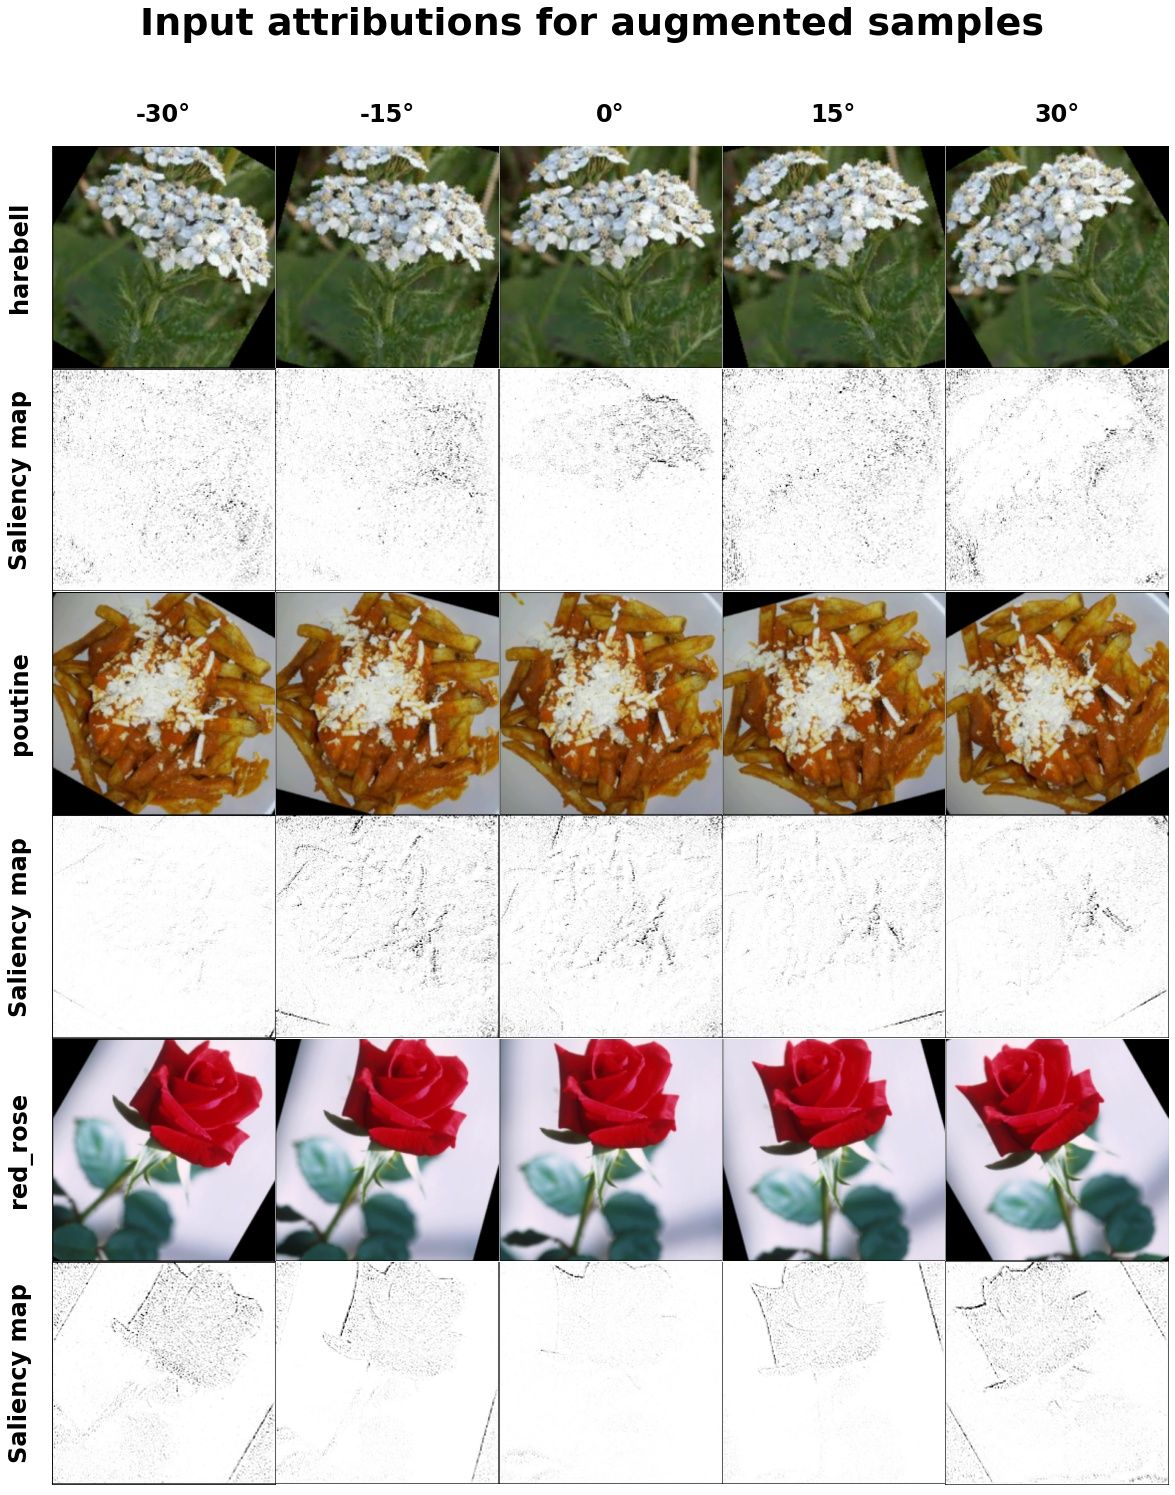
\includegraphics[width=0.8\textwidth]{appendixes/images/rotation-sample.jpg}
  \caption{\textbf{Attribution comparison of rotated inputs.} Figure shows three distinct images (\textit{harebell\_flower}, \textit{poutine}, \textit{red\_rose}) with different rotations. All attributions done by Guided GradCAM.}\label{fig:rotation-samples}
\end{figure}